\documentclass[10pt]{beamer}

\usetheme{metropolis}
\usepackage{appendixnumberbeamer}

\usepackage{booktabs}
\usepackage[scale=2]{ccicons}

\usepackage{pgfplots}
\usepgfplotslibrary{dateplot}

\usepackage{xspace}
\newcommand{\themename}{\textbf{\textsc{metropolis}}\xspace}

\usepackage{url}
\usepackage{courier}
\usepackage[skip=5pt]{caption}
\usepackage{xcolor}
\usepackage{framed}
\usepackage{float}
\usepackage{listings}

\definecolor{groovyblue}{HTML}{0000A0}
\definecolor{groovygreen}{HTML}{008000}
\definecolor{regexcolor}{HTML}{003300}
\definecolor{comment}{HTML}{B22400}
\definecolor{functions}{HTML}{660000}

\lstdefinelanguage{Groovy}[]{Java}{
  basicstyle=\ttfamily,
  columns=fixed,
  keywords=[3]{def, new, as, in, use, each, grep, inject, INVASIVE, CANCER, LOBULAR, DUCTAL, \$A, \$N},
  keywords=[4]{select, create, match, process, code, text},
  keywords=[5]{Sentence, CancerFinding, PostNegationTerm, PreNegationTerm, DictMatch, Token, AnnotationRegex, HistoryTerm},
  keywordstyle=[3]\bfseries,
  keywordstyle=[4]\color{functions}\bfseries,
  keywordstyle=[5]\color{groovyblue}\bfseries,
  stringstyle=\color{groovygreen}\ttfamily,
  commentstyle=\color{comment},
  moredelim=[is][\textcolor{groovyblue}]{\%\%}{\%\%},
  xleftmargin=0em,
  literate={~} {$\sim$}{1},
  aboveskip=0pt,
  belowskip=-5pt
}
\lstset{language=Groovy}

\newcommand{\DSLAnnotator}{\texttt{DSL\_Annotator}}

%------------------------------------------------------------------------------
\title{Natural Language Processing}
\subtitle{Regular Expressions and Beyond}
\date{February 22, 2019}
\author{Will Thompson, Ph.D.}
% \institute{Center for modern beamer themes}
% \titlegraphic{\hfill\includegraphics[height=1.5cm]{logo.pdf}}
%------------------------------------------------------------------------------

\begin{document}

\maketitle

%------------------------------------------------------------------------------
\begin{frame}{Table of contents}
  \setbeamertemplate{section in toc}[sections numbered]
  \tableofcontents[hideallsubsections]
\end{frame}
%------------------------------------------------------------------------------

\section{Introduction}

%------------------------------------------------------------------------------
\begin{frame}[fragile]{NLP: What is it and what is it good for?}
\begin{itemize}
  \item Text exploration (keyphrases, topic models)
  \item Text classification (including sentiment analysis)
  \item Information Extraction (unstructured to structured)
\end{itemize}
\end{frame}
%------------------------------------------------------------------------------

\section{Regular Expressions}

%------------------------------------------------------------------------------
\begin{frame}[fragile]{Regular Expressions: Hands On Demo}

\begin{center}
  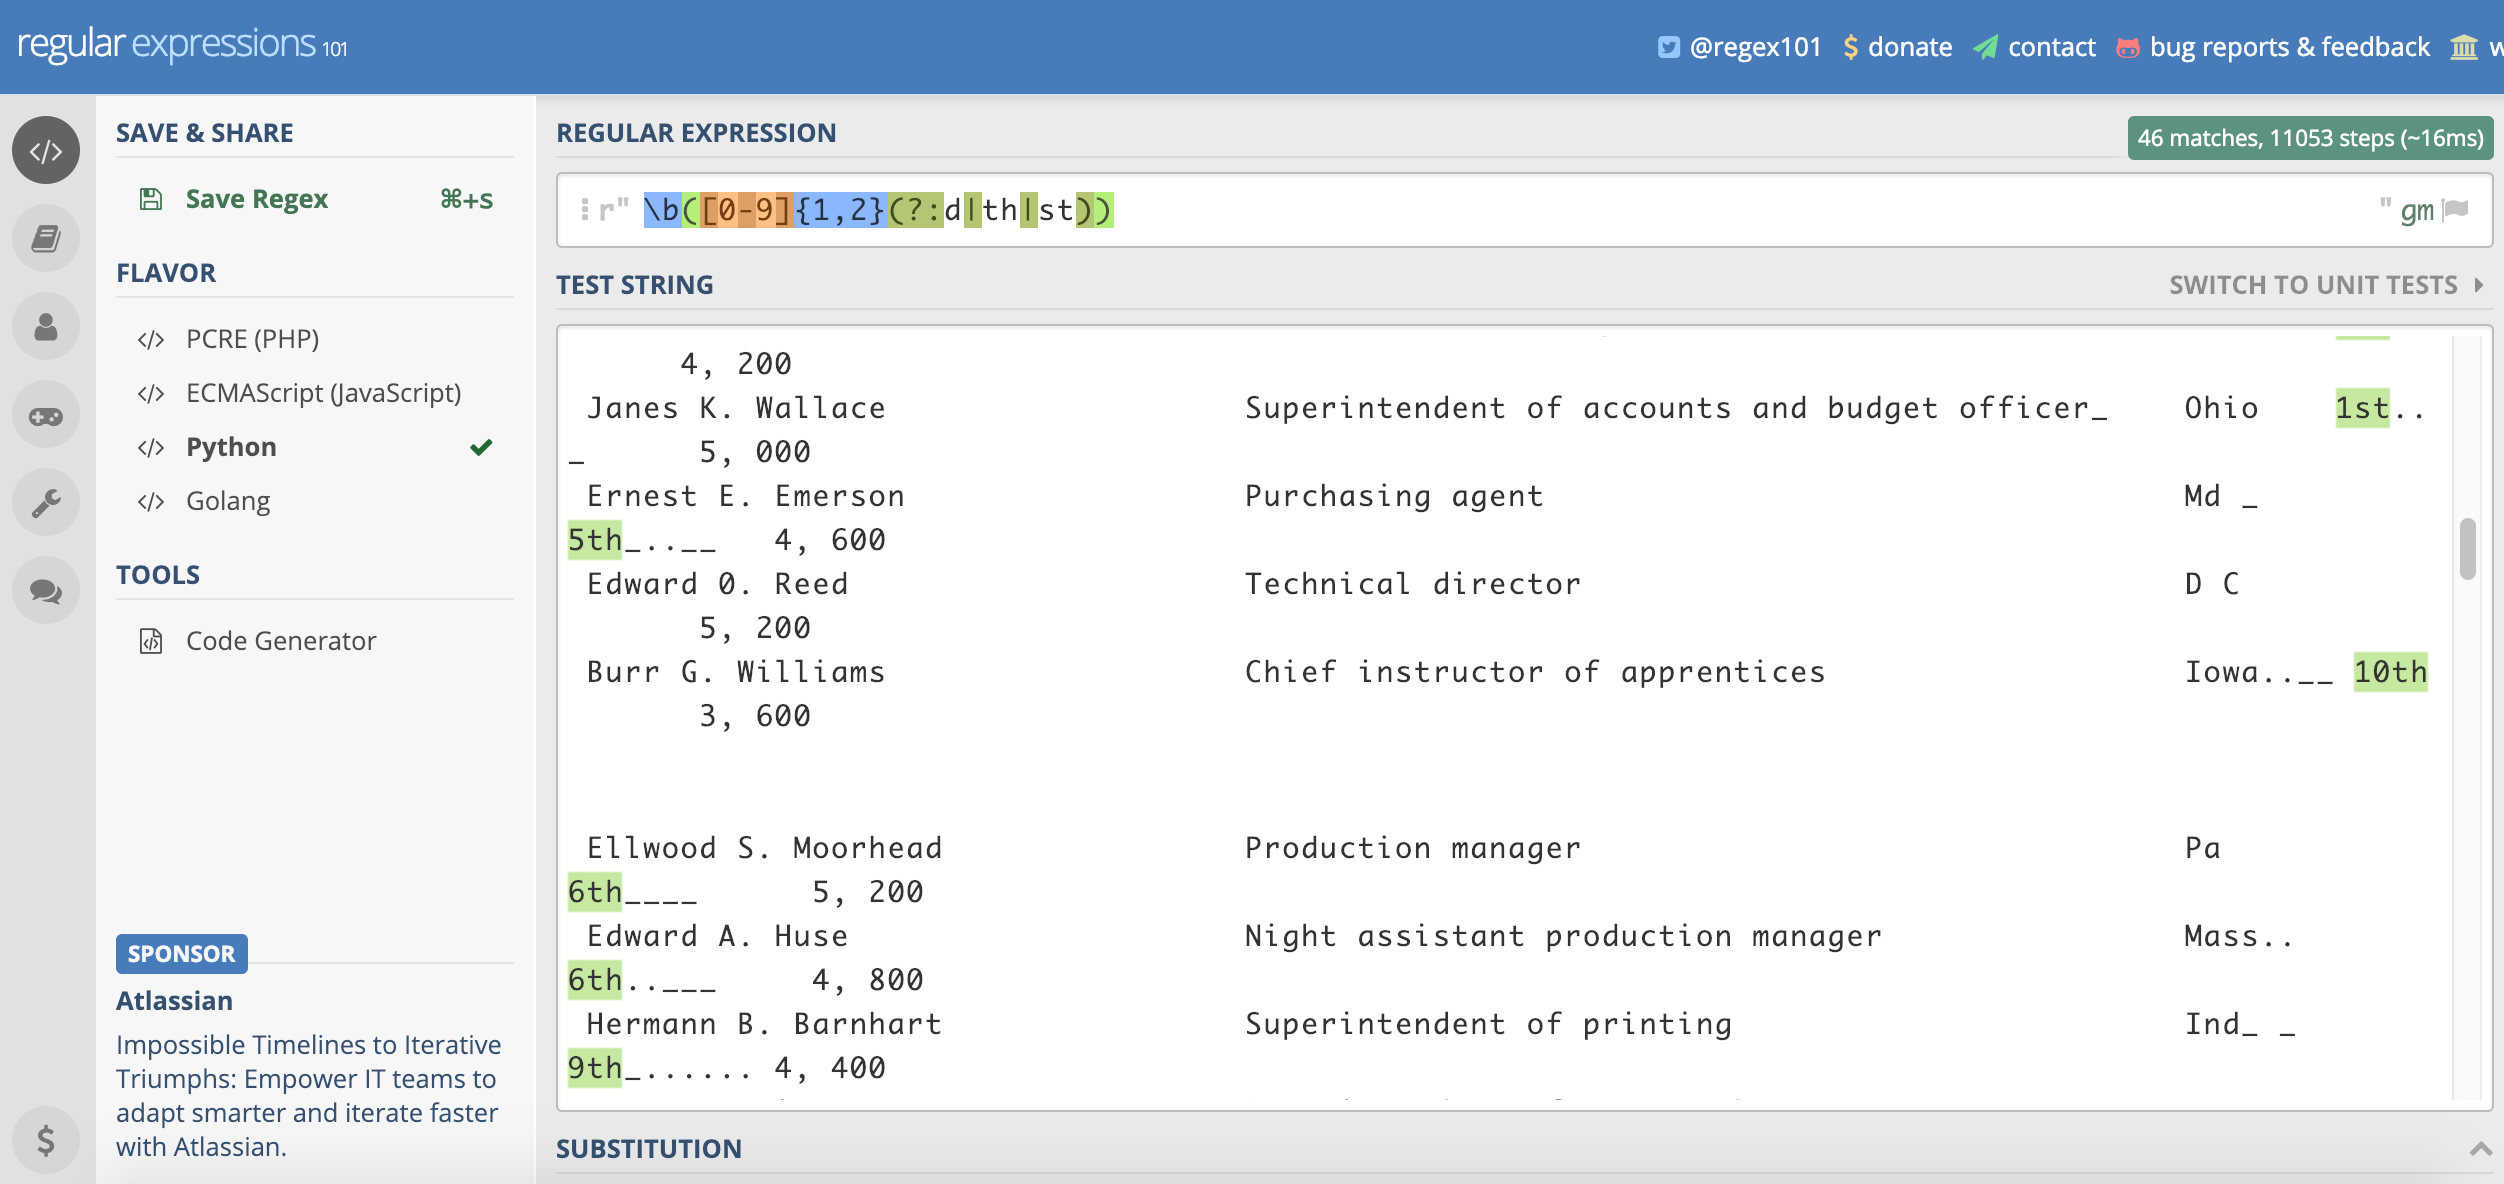
\includegraphics[scale=0.25]{figures/regex101-screenshot.png}
  \\ \vspace{1em}
  \textcolor{blue}{\url{https://regex101.com/}}
  \\
  (For fun: \textcolor{blue}{\url{https://regexcrossword.com/}})
\end{center}

\end{frame}
%------------------------------------------------------------------------------

%------------------------------------------------------------------------------
\begin{frame}[fragile]{Annotation Pattern Matching}

\begin{lstlisting}[frame=single]
def regex = new AnnotationRegex(
 (DictMatch, [code:INVASIVE])
 (DictMatch, [code:CANCER])
 ( (Token, [text:/with|having|/])(0,1)
   (DictMatch, [code:LOBULAR|DUCTAL)
   (Token, [text:/features/]) )(0,1)
)
\end{lstlisting}

\begin{itemize}
	\item There are still too many possible phrasings to easily create an exhaustive dictionary
	\item Solution: create \alert{patterns} over annotations
	\item Patterns that match a sequence of annotations trigger \alert{actions}, such as generating higher-level annotations.
\end{itemize}

\end{frame}
%------------------------------------------------------------------------------

%------------------------------------------------------------------------------
\begin{frame}[fragile]{Contextual Attributes: Negation and History}
\begin{lstlisting}[frame=single]
def regex = new AnnotationRegex(
 (CancerFinding)
 (Token)(0,5)
 (PostNegationTerm)
\end{lstlisting}

\begin{lstlisting}[frame=single]
def regex = new AnnotationRegex(
 (PreNegationTerm)
 (Token)(0,5)
 (CancerFinding)
\end{lstlisting}

\begin{lstlisting}[frame=single]
def regex = new AnnotationRegex(
 (HistoryTerm)
 (Token)(0,5)
 (CancerFinding)
\end{lstlisting}

\end{frame}
%------------------------------------------------------------------------------

\section{Advanced NLP: spaCy and textacy}

%------------------------------------------------------------------------------
% \begin{frame}[fragile]{Jupyter Notebook Demo}
%
% \end{frame}
%------------------------------------------------------------------------------


\end{document}
